\begin{filecontents*}{presentation.bib}
@article{Kaelin:2005gm,
	author = {Kaelin, William G},
	title = {{The concept of synthetic lethality in the context of anticancer therapy.}},
	journal = {Nat. Rev. Cancer},
	year = {2005}
}
@article{thanei2018xyz,
	title={The xyz algorithm for fast interaction search in high-dimensional data},
	author={Thanei, Gian-Andrea and Meinshausen, Nicolai and Shah, Rajen D},
	journal={The Journal of Machine Learning Research},
	volume={19},
	number={1},
	pages={1343--1384},
	year={2018},
	publisher={JMLR. org}
}
\end{filecontents*}

\documentclass[8pt]{beamer}
\usetheme{Hannover}

\usepackage[style=numeric,firstinits=true,backend=biber]{biblatex}
\addbibresource{presentation.bib}
\usepackage{todonotes}

\presetkeys{todonotes}{inline}{}

%\geometry{paperwidth=140mm,paperheight=105mm}

\title{Inferring Genetic Interactions Using xyz}
\author{Kieran Elmes}
\begin{document}
\begin{frame}[plain]
    \maketitle
\end{frame}

\section{Background}
\begin{frame}{The Problem}
\begin{minipage}{0.4\linewidth}
	\includegraphics[width=0.8\linewidth]{"cells_2x"}\\[-1ex]
	{\tiny Obligatory xkcd\\Source: \href{https://www.xkcd.com/1217/}{https://www.xkcd.com/1217/}}
\end{minipage}%
\begin{minipage}{0.6\linewidth}
	\begin{itemize}
		\item Killing cancer cells is easy. Killing cancer cells selectively is hard.
		\item Synthetic lethal interactions could potentially be used for exactly that.\cite{Kaelin:2005gm}
		\item We have approx. 20,000 genes. Experimentally testing all 200 million pairwise interactions is awkward.
	\end{itemize}
\end{minipage}
\end{frame}

\begin{frame}{What are we doing}
\begin{itemize}
	\item Simulating large(ish) sets of SiRNA knockdowns, and measuring xyz's ability to correctly determine interactions in the data.
	\item We can already do this with glinternet, but xyz is (several hundred times?) faster.
	\item xyz $= O(p^\alpha)$ for $1 < \alpha < 2$, depending on the strength of the interactions.
\end{itemize}
\end{frame}

\begin{frame}{The Data}
\begin{itemize}
	\item SiRNAs can reduce the expression of several hundred genes at once.
	\item $X \leftarrow n \times p$ matrix, $n$ trials with $p$ affected genes.
	\item $Y \leftarrow p$ fitness values.
\end{itemize}
\end{frame}

\begin{frame}{glinternet}
\centering
	\begin{itemize}
		\item Fits the data with a group-lasso.
	\end{itemize}
	\begin{minipage}{0.8\linewidth}
		\centering
		\includegraphics[width=\linewidth]{"PrecRecF1/glinternet_figure"}
	\end{minipage}
\end{frame}

\begin{frame}{xyz}
	\begin{itemize}
		\item Converts $X, Y$ into an equivalent matrix $Z = (z_1,z_2,...)$, which is then projected into a single dimensional space, in a way that mostly preserves closeness.
		\item Find now close points, rinse and repeat.
	\end{itemize}
	~\\
	\begin{minipage}{\linewidth}
		\centering
		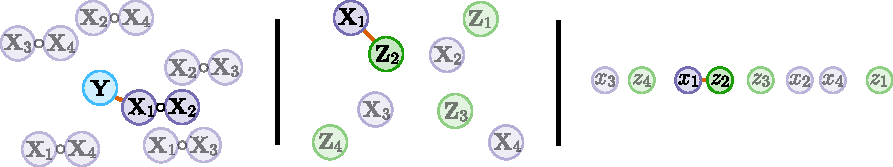
\includegraphics[width=0.7\linewidth]{xyz_explanation}
		{Source: \cite{thanei2018xyz}}
	\end{minipage}
\end{frame}

\begin{frame}{Runtime comparison}
\centering
	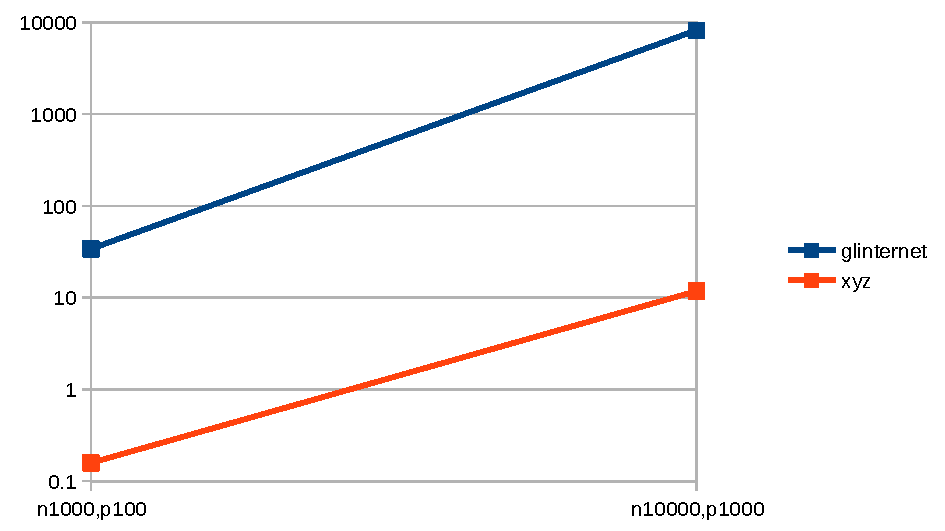
\includegraphics[width=0.75\linewidth]{time_comparison}
	\\~\\~
	The slow time for glinternet is actually the time it took for me to give up.
\end{frame}

\section{Simulation}
\begin{frame}{$P = 100$}
Results for $p=100$ using vanilla xyz
\begin{center}
\begin{minipage}{0.9\linewidth}
	\centering
	\includegraphics[width=0.5\linewidth]{"PrecRecF1/PrecRecF1_n1000_tno-vanilla_xyz"}%
	\includegraphics[width=0.5\linewidth]{"PrecRecF1/PrecRecF1_n1000_tyes-vanilla_xyz"}
\end{minipage}
\end{center}
For 1000 measurements of only 100 genes, this works.
\end{frame}
\begin{frame}{$P = 1000$}
Results for $p=1000$ using vanilla xyz
\begin{center}
	\begin{minipage}{0.9\linewidth}
		\centering
		\includegraphics[width=0.5\linewidth]{"PrecRecF1/PrecRecF1_n10000_tno-vanilla_xyz"}%
		\includegraphics[width=0.5\linewidth]{"PrecRecF1/PrecRecF1_n10000_tyes-vanilla_xyz"}
	\end{minipage}
\end{center}
Large data sets are a problem, however.
\end{frame}
\begin{frame}{$P = 1000$, increased limits in xyz}
Results for $p=1000$ using increased limits\footnote{commit 4517afbc59bdf091eed75683a28070476933f5da}
\begin{center}
	\begin{minipage}{0.85\linewidth}
		\centering
		\includegraphics[width=0.5\linewidth]{"PrecRecF1/increased_limits/PrecRecF1_n10000_tno"}%
		\includegraphics[width=0.5\linewidth]{"PrecRecF1/increased_limits/PrecRecF1_n10000_tyes"}
	\end{minipage}
\end{center}
Increasing the maximum allowed number of interactions in xyz does not improve results.
\end{frame}

\begin{frame}{Larger values of $L$}
\begin{center}
	\begin{minipage}{0.5\linewidth}
		\centering
		\includegraphics[width=0.9\linewidth]{"l_diff/quant_analysis_n10000"}
	\end{minipage}%
	\begin{minipage}{0.1\linewidth}
		\ 
	\end{minipage}%
	\begin{minipage}{0.4\linewidth}
		\begin{itemize}
			\item $L = 1000$ produces a smaller set of results than $L=100$, with similar accuracy.
			\item For our purposes $L = 100$ will be used from now on.
		\end{itemize}
	\end{minipage}
\end{center}

\end{frame}
\begin{frame}{Larger values of $L$, $SNR = 5$}
\begin{center}
	\begin{minipage}{0.9\linewidth}
		\centering
		\includegraphics[width=0.5\linewidth]{"l_diff/l_diff_n10000_SNR5_tno"}%
		\includegraphics[width=0.5\linewidth]{"l_diff/l_diff_n10000_SNR5_tyes"}
	\end{minipage}
\end{center}

\end{frame}

\begin{frame}{Interaction strength}
\begin{center}
	\begin{minipage}{0.9\linewidth}
		\centering
		\includegraphics[width=0.5\linewidth]{"FXstrength/FXstrength_PRF_n10000_L100_tno_mult10"}%
		\includegraphics[width=0.5\linewidth]{"FXstrength/FXstrength_PRF_n10000_L100_tyes_mult10"}
	\end{minipage}
\end{center}

A small number of strong interactions seems best.
\end{frame}


\begin{frame}{Large data, few interactions}
	\begin{minipage}{0.9\linewidth}
		\centering
		\includegraphics[width=0.5\linewidth]{"PrecRecF1/PrecRecF1_n10000_tno_large0"}%
		\includegraphics[width=0.5\linewidth]{"PrecRecF1/PrecRecF1_n10000_tyes_large0"}
	\end{minipage}\\
	Performance is similar with only a few interactions in a large data set.
\end{frame}

\begin{frame}
	\begin{minipage}{0.9\linewidth}
		\centering
		\includegraphics[width=0.5\linewidth]{"FXstrength/FXstrength_PRF_n10000_L100_tno_mult1"}%
		\includegraphics[width=0.5\linewidth]{"FXstrength/FXstrength_PRF_n10000_L100_tyes_mult1"}
	\end{minipage}

	With only a few interactions, xyz is able to find strong interactions much more easily.
\end{frame}

\begin{frame}{Synthetic Lethal Pairs}
	\begin{minipage}{0.9\linewidth}
		\centering
		\includegraphics[width=0.5\linewidth]{"PrecRecF1/PrecRecF1_n10000_tno_large0_lethal"}%
		\includegraphics[width=0.5\linewidth]{"PrecRecF1/PrecRecF1_n10000_tyes_large0_lethal"}
	\end{minipage}

	(Work in progress, there's a chance these were not generated correctly)
\end{frame}

\begin{frame}{Summary}
\begin{itemize}
	\item xyz may be useful for finding strong interactions, but it's not looking good.
\end{itemize}
\end{frame}

\begin{frame}{WIP/TODO}
\begin{itemize}
	\item Test detection of synthetic lethal pairs specifically, including glinternet.
	\item Re-run without imposing a strong hierarchy for the sake of glinternet.
\end{itemize}
\end{frame}

\begin{frame}
\frametitle{References}
\printbibliography
\end{frame}
\end{document}



% Things to mention: (also see notes)
